% pdflatex rapport.tex; pdflatex rapport.tex; pdflatex rapport.tex
\documentclass[a4paper]{article}

\usepackage[francais]{babel}
\usepackage[utf8]{inputenc}
\usepackage{amsmath}
\usepackage{amssymb}
\usepackage{graphicx}
\usepackage{algorithmic}
\usepackage{url}
\usepackage{subfigure}
\usepackage[squaren,Gray]{SIunits}

% shorten margin
\usepackage[]{fullpage}

\title{Création d'un framework pour des routeurs
	avec support pour notification de vitesse explicite
	(kernel space)\\Encadrant: Dino Lopez}
\author{Calypso Petit, François Chapuis, Sophie Valentin, Mathieu Bivert}

\begin{document}
\maketitle
\tableofcontents

\section{Introduction}
L'essor de réseaux de grande envergure nécessite la mise en
place de protocoles de contrôle de congestion. En effet,
l'augmentation du traffic, et la distribution non-équitable
des ressources entre les usagers, peuvent conduire à un
ralentissement des communications.

Une famille de protocoles de contrôle de congestion est l'IP-ERN
(Explicit Rate Notification). Ils reposent sur les informations
envoyées/calculées par des routeurs, comme le taux d'émission
optimal. Dans le cadre de notre projet, nous devons élaborer un
module noyau à destination d'un routeur supportant l'IP-ERN.
Un tel protocole modifie les paquets TCP transitant par le
routeur.Dans un premier temps, nous allons élaborer des statistiques
sur les paquets TCP qui traversent le routeur. Puis dans un
second temps, nous nous attarderons sur le protocole (ou pas).

\section{Description du problème}
\subsection{Contexte}
Un routeur est une machine qui assure l’acheminement des données,
d'un réseau informatique à un autre. Son rôle consiste à diriger
les paquets d'une interface réseau vers une autre par le chemin
le plus rapide et selon les règles définies dans la table de
routage. Les interfaces réseaux peuvent être assimilées à des
portes par lesquelles les données entrent et sortent du routeur, et
la table de routage à une façon de diriger les paquets à travers
ces portes. Il s'agit ici dans un premier temps de calculer
des statistiques nécessaires pour le protocole IP-ERN.

\subsection{Netfilter}
Netfilter est un framework permettant l'interception des paquets
grâce à des hooks : ce sont des points d'accroche dans le noyau.
Lorsqu'un événement réseau se produit (entrée d'un paquet par exemple),
une fonction de callback associée à ce type d'évènement est appelée.
A chaque hook, Netfilter permet d'accepter les paquets ou de s'en
débarasser. Pour le protocole IPv4, on compte cinq hooks. Ces derniers
sont organisés comme sur \ref{hooks}.

\begin{figure}[!ht]
	\centering
	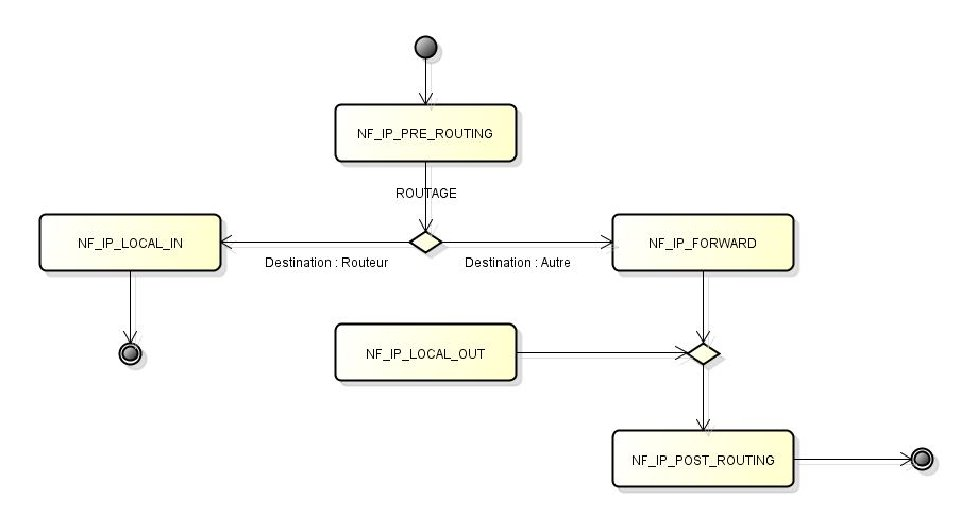
\includegraphics[scale=.5]{hooks.jpg}
	\caption{\label{hooks} Position des Hooks netfilter}
\end{figure}

Les paquets entrent par le haut. Après avoir subi des tests au
niveau de la carte réseau, ils traversent un premier hook, appelé
hook \textit{NF\_IP\_PRE\_ROUTING}. À ce niveau, seule l'interface
d'entrée du routeur est connue. Ensuite, après consultation de
la table de routage, les paquets à destination du routeur sont
dirigés vers un processus interne et passent par le deuxième hook,
\textit{NF\_IP\_LOCAL\_IN}. Quant aux autres paquets, ils sont dirigés
vers une interface de sortie et traversent successivement le troisième
hook, \textit{NF\_IP\_FORWARD} puis le quatrième,
\textit{NF\_IP\_POST\_ROUTING}. Au niveau du troisième hook, les
interfaces d'entrée et sortie sont connues. En revanche, dans
le quatrième, seule l'interface de sortie est connue.

En utilisant l'architecture de Netfilter, nous devons renseigner
un tableau de statistiques comportant, pour chaque interface, le
nombre de paquets entrants à destination de cette interface
(Input trafic Rate, \textit{I}) et le nombre de paquets sortants
(Output trafic Rate, \textit{O}) par cette interface. La quantité
de donnée pouvant circuler sera donnée par l'Output Link Capacity
(\textit{C}). Le tableau sera de la forme donnée par \ref{stats}.

\begin{figure}
	\centering
	\begin{tabular}{c|c|c|c|c}
		Nom de l'interface & I & O & C & Q = O-I \\
		\hline
		eth$0$ & $\ldots$ & $\ldots$ & $\ldots$ & $\ldots$ \\
		eth$1$ & $\ldots$ & $\ldots$ & $\ldots$ & $\ldots$ \\
		$\ldots$ & $\ldots$ & $\ldots$ & $\ldots$ & $\ldots$ \\
		eth$n$ & $\ldots$ & $\ldots$ & $\ldots$ & $\ldots$ \\
	\end{tabular}
	\caption{\label{stats} Statistiques requises par le protocole}
\end{figure}

En comptabilisant l'Input trafic Rate et l'Output trafic Rate,
on pourra déterminer la taille de la file d'attente (Qsize).
Cependant, ne sachant pas où ce buffer se situe, le choix des
hooks va être crucial.

Afin d'utiliser Netfilter, il faut programmer en mode noyau.
Les modules sont des morceaux de code écrits en langage C, pouvant
être ajoutés ou retirés du noyau dynamiquement. Ils apportent de
nouvelles fonctionnalités au noyau. Dans notre cas, le module
fournira des statistiques sur la taille de la file d'attente.
La programmation en mode noyau sous Linux est différente de celle
en mode utilisateur. En effet, les bibliothèques sont plus
restreintes et le débogage plus ardu, car le moindre accès
mémoire invalide peut rendre le système inutilisable.

L'utilisation de machines virtuelles permet donc d'éviter de
devoir redémarrer à chaque plantage, et va aussi faciliter
la mise en place d'interfaces réseaux, donc les tests de
façon générale.

Les détails techniques concernant la programmation de
modules Linux sont évoqués en annexe.

\section{Solutions}
\subsection{Environnement de tests}
Dans un premier temps, on souhaite mettre en place une
architecture réseau simple, constituée de trois machines, la
figure \ref{topo} indiquant la topologie réseau suivie:
\begin{itemize}
	\item un émetteur;
	\item un routeur;
	\item et un récépteur.
\end{itemize}

\begin{figure}[!ht]
	\centering
	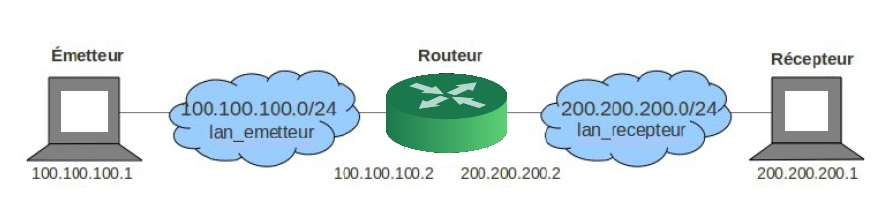
\includegraphics[scale=.5]{topo.jpg}
	\caption{\label{topo} Topologie du réseau}
\end{figure}

Pour cela, nous utilisons trois machines virtuelles,
lancées sur la même machine. Virtualbox met à disposition
plusieurs d'interfaces réseaux virtuelles:
\begin{description}
	\item[NAT] interface connectée à un réseau local, sur\
	lesquelles se trouvent les différentes machines virtuelles
	\item[Bridge] interface connectée au réseau de la machine hôte
\end{description}

Un routeur servant à faire transiter des données d'un réseau
à un autre, il nous en faut donc deux : un sur lequel se
trouve l'émetteur, un pour le récepteur, et le routeur est
connecté au deux (fig.\ref{reseaux}).
\begin{figure}
	\centering
	\begin{tabular}{c|c|c}
	Nom du réseau & CIDR & Masque de sous-réseau\\
	lan\_emetteur & 100.100.100.0/24 & 255.255.255.0\\
	lan\_recepteur & 200.200.200.0/24 & 255.255.255.0\\
	\end{tabular}
	\caption{\label{reseaux} Les deux réseaux}
\end{figure}

Il faut donc configurer sur chaque machine les interfaces
réseaux NAT en conséquence, ainsi qu'ajouter des entrées
dans la table de routage au niveau de l'émetteur et
du récépteur.

Le routeur doit simplement être connecté aux deux réseaux.
Chacune des deux interfaces du routeur doit donc être
connectée au bon réseau:
\begin{verbatim}
  # ifconfig eth1 100.100.100.2 netmask 255.255.255.0
  # ifconfig eth2 200.200.200.2 netmask 255.255.255.0
\end{verbatim}

Enfin, il ne faut pas oublier d'activer le transfert de
paquets :
\begin{verbatim}
  # echo 1 > /proc/sys/net/ipv4/ip_forward
\end{verbatim}

Du côté de l'émetteur, l'interface eth$0$ est reliée à
\textit{lan\_emetteur}, et il faut passer par 100.100.100.2
(c'est-à-dire l'interface eth$1$ du routeur) pour transmettre
des paquets à destination du réseau lan\_recepteur:
\begin{verbatim}
  # ifconfig eth0 100.100.100.1 netmask 255.255.255.0
  # route add -net 200.200.200.0 netmask 255.255.255.0 gw 100.100.100.2 eth0
\end{verbatim}

Côté récepteur, la configuration est analogue à celle de l'émetteur:
\begin{verbatim}
  # ifconfig eth0 200.200.200.1 netmask 255.255.255.0
  # route add -net 100.100.100.0 netmask 255.255.255.0 gw 200.200.200.2 eth0
\end{verbatim}

\subsection{Test de connectivité}
En guise de vérification, on essaye de \textit{pinger} le
récépteur depuis l'émetteur (fig.\ref{ping}):
\begin{figure}
	\centering
	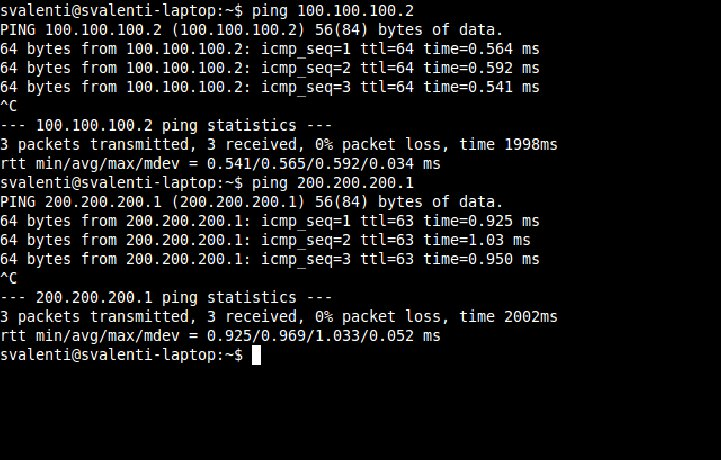
\includegraphics[scale=.5]{ping.jpg}
	\caption{\label{ping} Émetteur et récépteur peuvent communiquer}
\end{figure}

La commande \textit{ping} n'est pas suffisante pour envoyer
des paquets dans le cadre de notre projet car elle utilise
le protocole ICMP et non le protocole IP. Par conséquent,
nous avons cherché un outil utilisant les protocoles IP et TCP.
(Est-ce qu’il faut spécifier ce que sont les protocoles IP et TCP ?)
La commande \textit{iperf} permet d'envoyer entre un client et
un serveur des paquets TCP ou UDP. Nous l'avons donc utilisé
entre l'émetteur et le récépteur. Par défaut \textit{iperf}
utilise le protocole TCP.

Côté récépteur, on lance \textit{iperf} en mode serveur:
\begin{verbatim}
  # iperf -s
\end{verbatim}

et côté émetteur, on envoie des paquets sur le récépteur:
\begin{verbatim}
  # iperf -c 200.200.200.1
\end{verbatim}

L'option \textit{-i} d'\textit{iperf} peut-être utilisée
pour fixer l'intervalle de temps entre les rapports
d'envois de paquets (mesure bande passante, $\ldots$).

\subsection{Détermination de la taille de la pile avec Netfilter}
A présent, nous écrivons un module utilisant Netfilter. Les
fonctions de callback données par les hooks permettent
d'accéder à un \textit{struct sk\_buff}. Cette structure représente
un paquet dans le noyau Linux. Il est ainsi possible de récupérer
les informations du datagramme telles que le protocole ou encore
l'adresse IP de destination.

Les fonctions de callback fournissent également deux structures
de type \textit{struct net\_device} : une pour l'interface réseau
d'entrée et une autre pour l'interface réseau de sortie. Avec
une telle structure, on peut connaître le nom de l'interface
grâce au champ \textit{net\_device.name}.

Cependant, ces structures ne sont pas toujours remplies par
le noyau : cela dépend du hook dans lequel nous nous trouvons.
Pour déterminer où se trouve la file d'attente, nous devons
travailler avec deux hooks : le premier hook doit se trouver
en amont de l'emplacement supposé de la file d'attente et le second
 en aval. Dans le premier hook, l'input trafic rate de l'interface
 de sortie est incrémenté et dans le second hook, l'output trafic
 rate de l'interface de sortie est incrémenté.
 
Après chaque opération, on met à jour la taille de la file
d'attente de l'interface de sortie en soustrayant l'input trafic
rate par l'output trafic rate.

Les deux hooks pouvant accéder aux mêmes données en même temps,
il est indispensable de mettre en place un mécanisme de
synchronisation. Les hooks étant déclenchés par des interuptions,
il est impossible d'utiliser des mutex ou encore des sémaphores.
Le noyau fourni des spinlocks, jouant le même  rôle, mais dans
un contexte d'interuptions.

Les hooks concernant les paquets qui traversent le routeur sont :
\textit{NF\_IP\_PRE\_ROUTING}, \textit{NF\_IP\_FORWARD} et
\textit{NF\_IP\_POST\_ROUTING}. Parmi ces hooks, seuls
\textit{NF\_IP\_FORWARD} et \textit{NF\_IP\_POST\_ROUTING}
contiennent l'information sur l'interface de sortie dans la
structure \textit{net\_device}. Par conséquent, nous allons
tout d'abords chercher la taille de la pile entre
\textit{NF\_IP\_FORWARD} et \textit{NF\_IP\_POST\_ROUTING}.

\subsubsection{\textit{NF\_IP\_FORWARD} et \textit{NF\_IP\_POST\_ROUTING}}
Pour commencer, les vitesses maximales des interfaces eth$1$ et
eth$2$ sont configurées de la même façon. Ainsi, on s'attend à
ce que la sortie des paquets soit fluide : nous ne nous attendons
pas à la création d'une file d'attente interne.L'exécution du module
utilisant ces deux hooks donne l'extrait de trace en
fig.\ref{forwardpost}.

\begin{figure}
	\centering
	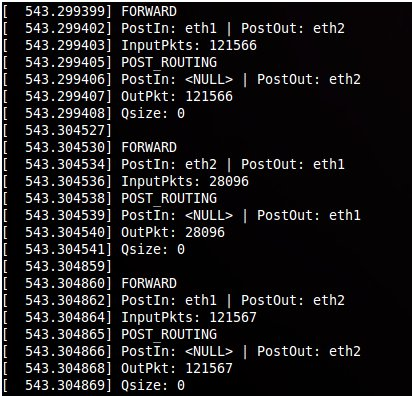
\includegraphics[scale=.5]{forward_post.jpg}
	\caption{\label{forwardpost} Trace obtenue entre FORWARD et ROUTING}
\end{figure}

Après examination entière de la trace, on constate que Qsize
pour eth$1$ et Qsize pour eth$2$ sont constamment égaux à zéro.
On peut tout de même vérifier que le nombre de paquets entrants
est incrémenté correctement à chaque exécution de la fonction
de callback de \textit{NF\_IP\_FORWARD}. Quant au nombre de paquets
sortants, il est incrémenté correctement à chaque exécution de la
fonction de callback du hook \textit{NF\_IP\_POST\_ROUTING}.

À présent, on configure la bande passante maximale de l'interface
eth$2$ afin que la vitesse maximale soit de $10$ Mbits/seconde.
Pour cela, on utilise la commande \textit{tc} (traffic control).
Cette commande va agir sur le fonctionnement des files d’attente
en sortie d’une interface donnée.
\begin{verbatim}
  # tc qdisc add dev eth2 root handle 1: tbf rate 10mbit buffer 1600 limit 3000
  # tc qdisc add dev eth2 parent 1: handle 10: netem delay 3ms
\end{verbatim}
Pour limiter la bande passante, on utilise un Token Bucket Filter
(tbf) en précisant qu’on ne peut pas dépasser un débit de
$10$Mbits/seconde.

Après avoir ainsi configuré la vitesse maximale,
nous nous attendons à obtenir une file d’attente non nulle.
Les résultats des tests effectués nous montrent que la taille
de la file d’attente est toujours nulle, ce qui prouve que la
file d’attente interne ne se trouve pas entre les hooks
\textit{NF\_IP\_FORWARD} et \textit{NF\_IP\_POST\_ROUTING}.

Il nous faut donc regarder entre deux autres hooks.

\subsubsection{\textit{NF\_IP\_PRE\_ROUTING} et \textit{NF\_IP\_POST\_ROUTING}}
L'interface de sortie n'étant plus disponible en PRE ROUTING,
il va nous falloir effectuer le routage à la main. Notre
objectif étant de chercher où se trouve la file, nous nous
contentons d'un routage manuelle, avec les valeurs entrées en
dur dans le code.

Nous obtenons finalement le même résultats qu'entre FORWARD et POST,
il semble donc qu'il soit impossible d'utiliser Netfilter pour
obtenir les statistiques. On pourrait cependant empiler les paquets
sur lesquelles on désire avoir des statistiques, et passer le
buffer en userspace pour y faire les calculs. Il est néamoins
important pour le code d'être efficace, et sortir du mode noyau
a de fortes chances d'impacter la vitesse d'exécution du code
(pourquoi?); on va donc chercher une autre façon d'obtenir
la taille de la pile tout en restant en mode noyau.

\subsection{Lecture des statistiques sur les cartes réseaux}
Grâce à une fonction du noyau, il est possible d’accéder à des
statistiques concernant les interfaces. La fonction \textit{dev\_get\_stats}
définie dans \textit{linux/netdevice.h} fournit :
\begin{itemize}
	\item le nombre de paquets (ou octets) reçus sur une interface;
	\item le nombre de paquets (ou octets) transmis par une interface;
	\item le nombre d’erreurs;- et le nombre de paquets “dropped”.
\end{itemize}

Ces statistiques pourraient nous aider à calculer Qsize. Cependant,
elles ne permettent pas de différencier les paquets TCP des autres paquets.
Il nous faut donc aller un peu plus loin dans le code.

\section{Localisation des files d'attente dans la couche liaison}
\subsubsection{npkt++}

\subsubsection{Wrapper pour les drivers ethernet (npkt--)}
Les fonctions permettant de manipuler une carte ethernet sont sous
linux abstraite par une structure : ajouter un driver revient donc
à déclarer une structure et à remplir les différents champs, avec
les fonctions adaptées à la carte.
La structure \textit{net\_device\_ops}, déclarée dans
\textit{linux/netdevice.h} joue ce rôle:
\begin{verbatim}
struct net_device_ops {
    int (*ndo_init)(struct net_device *dev);
    void (*ndo_uninit)(struct net_device *dev);
    int (*ndo_open)(struct net_device *dev);
    int (*ndo_stop)(struct net_device *dev);
    netdev_tx_t (*ndo_start_xmit) (struct sk_buff *skb, struct net_device *dev);
    ...
};
\end{verbatim}

Et un driver, par exemple e1000, l'utilise ainsi:
\begin{verbatim}
static const struct net_device_ops e1000_netdev_ops = {
    .ndo_open               = e1000_open,
    .ndo_stop               = e1000_close,
    .ndo_start_xmit         = e1000_xmit_frame,
    .ndo_get_stats          = e1000_get_stats,
    ...
};
\end{verbatim}

La fonction \textit{dev\_hard\_start\_xmit}, située dans
\textit{net/core/dev.c}, est chargée de transmettre le paquet
à la carte. Après quelques tests à l'aide de \textit{printk} bien
placé, nous avons constaté que dans tous les cas, la fonction
est appellée, plus ou moins directement, et qu'elle contient 
un appel à \textit{ndo\_start\_xmit}. La décrementation de la
taille de la pile peut donc être effectuée ici, plutôt que de
l'être dans le noyau.

\section{Bibliographie}

\newpage
\appendix

\section{Compléments sur la programmation de modules Linux}
\subsection{Organisation générale}
\subsection{Mise en place d'un hook netfilter}
\subsection{Synchronisation (spinlock)}
\subsection{Compilation d'un noyau Linux}

\end{document}
